\documentclass{article}

\usepackage[english]{babel}
\usepackage{float}
\usepackage[letterpaper,top=2cm,bottom=2cm,left=3cm,right=3cm,marginparwidth=1.75cm]{geometry}
\usepackage{amsmath}
\usepackage{amssymb}
\usepackage{graphicx}
\usepackage{grffile}
\usepackage{booktabs}
\usepackage{array}
\usepackage{tabularx}
\usepackage{caption}
\usepackage{verbatim}
\captionsetup[figure]{justification=centering}
\usepackage[colorlinks=true, allcolors=blue]{hyperref}
\setlength{\emergencystretch}{3em}

\title{\textbf{ME 144L LE 8: Vision-Based Measurement with OpenCV}}
\author{Alejandro Diaz \\ TA: Gabrielle Naquila}
\date{April 6, 2026}

\begin{document}
\maketitle

% ============================================================
\section{Finding Theta from Coordinates}
% ============================================================

\subsection{Three-Point Model and Coordinate Setup}

The script \texttt{2\_click\_and\_save\_xy.py} measures a joint angle from three manually selected points on an image. Figure 1 shows the  model, which consists of two links joined at a central point. The angle of interest is the interior angle at the vertex between the two link directions.

\begin{figure}[H]
    \centering
    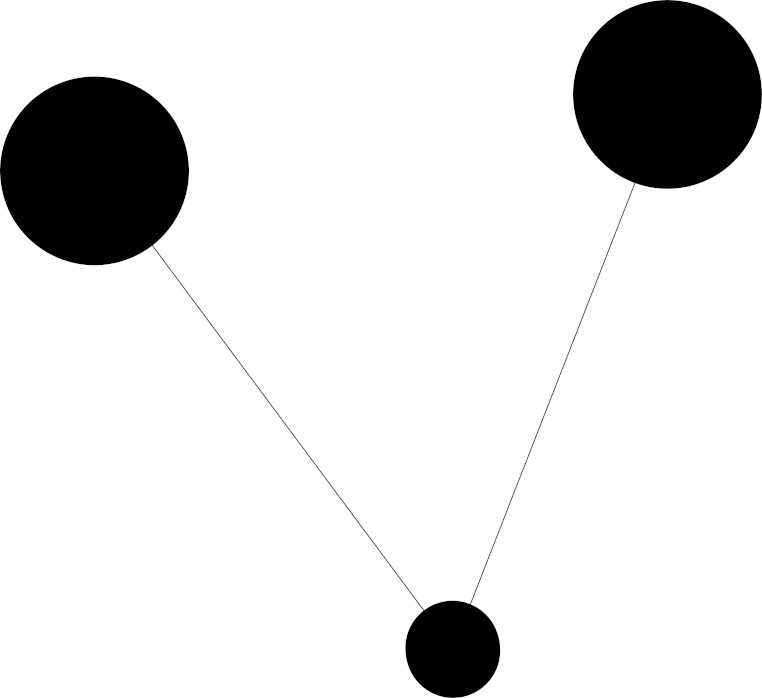
\includegraphics[width=0.5\linewidth]{figures/example_two_positions.jpg}
    \caption{Three-circle linkage model used for angle measurement.}
    \label{fig:two_positions}
\end{figure}

\subsection{Vector Definition}

\noindent The three clicked pixel coordinates be defined as:
\begin{align}
    P_\text{ref} = (x_r,\, y_r) \\
    P_\text{vertex} = (x_v,\, y_v) \\
    P_\text{pos}  = (x_p,\, y_p)
\end{align}
    
\noindent Two vectors are created from the vertex outward along each link:
\begin{align}
    \vec{v}_1 &= P_\text{ref} - P_\text{vertex} \\
    \vec{v}_2 &= P_\text{pos} - P_\text{vertex}
\end{align}

\noindent The vectors point from the pivot toward each endpoint, defining the two line directions in (x,y) coordinates. The angle $\theta$ at the vertex is the angle between $\vec{v}_1$ and $\vec{v}_2$. The dot product relates these two vectors to $\theta$, as shown in the following equation:

\begin{equation}
    \vec{v}_1 \cdot \vec{v}_2 = |\vec{v}_1|\,|\vec{v}_2|\cos\theta
\end{equation}

\noindent Solving for $\theta$:

\begin{equation}
    \theta = \arccos\!\left(\frac{\vec{v}_1 \cdot \vec{v}_2}{|\vec{v}_1|\,|\vec{v}_2|}\right)
    \label{eq:theta}
\end{equation}

\noindent Expanding to 2D components, the numerator dot product becomes:

\begin{equation}
    \vec{v}_1 \cdot \vec{v}_2 = (x_r - x_v)(x_p - x_v) + (y_r - y_v)(y_p - y_v)
\end{equation}

\noindent and the denominator magnitudes are:

\begin{equation}
    |\vec{v}_1| = \sqrt{(x_r - x_v)^2 + (y_r - y_v)^2}, \qquad
    |\vec{v}_2| = \sqrt{(x_p - x_v)^2 + (y_p - y_v)^2}
\end{equation}

\noindent Substituting into Equation 7:

\begin{equation}
    \theta = \arccos\!\left(
        \frac{(x_r - x_v)(x_p - x_v) + (y_r - y_v)(y_p - y_v)}
             {\sqrt{(x_r-x_v)^2+(y_r-y_v)^2}\;\sqrt{(x_p-x_v)^2+(y_p-y_v)^2}}
    \right)
    \label{eq:theta_full}
\end{equation}
\\
\noindent The script implements this seamlessly using \texttt{np.dot}, \texttt{np.linalg.norm}, and \texttt{np.arccos}, which defaults the angle output to radians. lastly, the \texttt{np.degrees} tool converts radians to degrees, resulting in the final interior angle of the linkage at the pivot joint. The output is always in the range $[0^\circ, 180^\circ]$.

% ============================================================
\section{Detecting Objects}
% ============================================================

\subsection{Preprocessing}

The script \texttt{5\_read\_cam\_detect\_circles.py} captures a webcam camera frame, then applies the Hough Circle Transform to detect circular objects. First, the frame is converted from BGR to grayscale, reducing the three-channel color image to a single intensity channel. A median blur with kernel size 5 is then applied, which helps suppress noise while preserving edge sharpness. Circle detection calls \texttt{cv2.HoughCircles} using the \texttt{HOUGH\_GRADIENT} method. Through experimental testing, the parameters used were tested to balance sensitivity and reduce false positives, which is shown in the table below.

\begin{table}[H]
    \centering
    \caption{Hough Circle Transform Parameters from \texttt{5\_read\_cam\_detect\_circles.py}}
    \label{tab:hough_params}
    \begin{tabular}{lll}
        \toprule
        \textbf{Parameter} & \textbf{Value} & \textbf{Effect} \\
        \midrule
        \texttt{dp}         & 1   & High resolution preset \\
        \texttt{minDist}    & 10  & Minimum distance between accepted circle centers \\
        \texttt{param1}     & 50  & Requirement for edge strength \\
        \texttt{param2}     & 40  & Confidence for accepting a circle \\
        \texttt{minRadius}  & 0   & No lower radius constraint \\
        \texttt{maxRadius}  & 0   & No upper radius constraint \\
        \bottomrule
    \end{tabular}
\end{table}

\noindent Figure 2 shows a screenshot of the circle detection output. The algorithm correctly identifies the five dots, drawing green circles that closely follow each dot's boundary. The green circles align closely with each dot's physical boundary, confirming the parameter values were tuned properly to detect all five targets without false positives.

\begin{figure}[H]
    \centering
    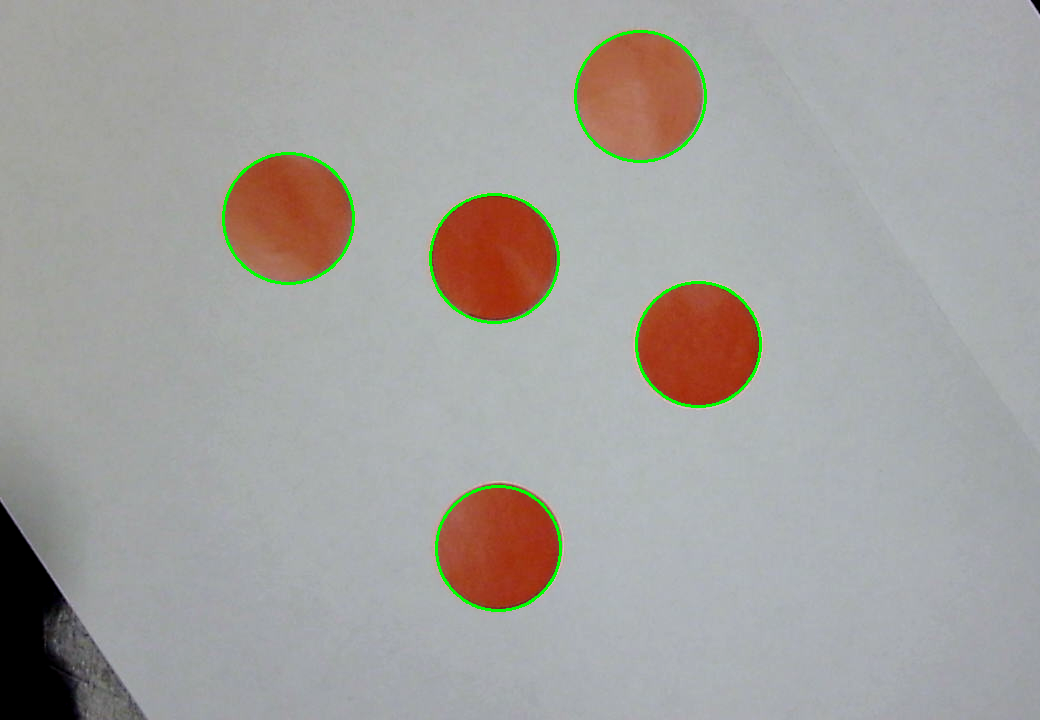
\includegraphics[width=0.65\linewidth]{figures/Detected_Circles_cropped.png}
    \caption{HoughCircles detection output (Green).}
    \label{fig:hough_circles}
\end{figure}

% ============================================================
\section{Tracking a Moving Dot}
% ============================================================

\subsection{Contour Detection Pipeline}

The script processes a pre-recorded video alongside a CSV of wall-clock timestamps from the recording session. Before per-frame processing begins, frame 30 is shown so the user can draw a region of interest with \texttt{cv2.selectROI}. That bounding box gets applied to every subsequent frame as a fixed crop, keeping irrelevant background out of the threshold step and setting the spatial extent used for scale calibration. This is useful as the ruler was positioned at the bottom of the frame, and would be cropped out by the ROI selection.

Each cropped frame is converted to grayscale, then threshold checked. First, the program uses \texttt{cv2.THRESH\_BINARY} at a tuned value of 20 to pull out bright areas. The second uses \texttt{cv2.THRESH\_BINARY\_INV} at 100, flipping the mask so dark pixels below intensity 100 become white foreground. Since the tracked dot is darker than the ruler background, the inverted threshold is used to isolate the circle. From the thresholded freame, \texttt{cv2.findContours} extracts outer boundaries, and the largest contour by area is kept.

\subsection{Parameter Tuning}

The two parameters tuned directly were the threshold values and \texttt{ruler\_length}. The inverted threshold at 100 controls which pixels are treated as foreground, and the value of 20 for the first binary pass was set to isolate the bright areas before the inversion. Both took some trial and error to tracked the dot cleanly across different parts of the frame without pulling in shadows or ruler markings.

The \texttt{ruler\_length} value of 9.5\,in sets the physical scale for the entire measurement. This was measured from the left edge of the ruler to right edge visible in the frame, and was established throughout the entire testing process by keeping the webcam position fixed.

Beyond the code parameters, the physical setup mattered just as much. Early runs picked up false contours from the paper edges, since any dark region that cleared the threshold competed with the dot and generated false positives. Placing the dot on a plain white sheet and using an extra paper as background removed most of those competing edges entirely. Figure 3 shows the final recording setup, with the single red dot on a white sheet providing a clean, high-contrast target against the neutral background.

\begin{figure}[H]
    \centering
    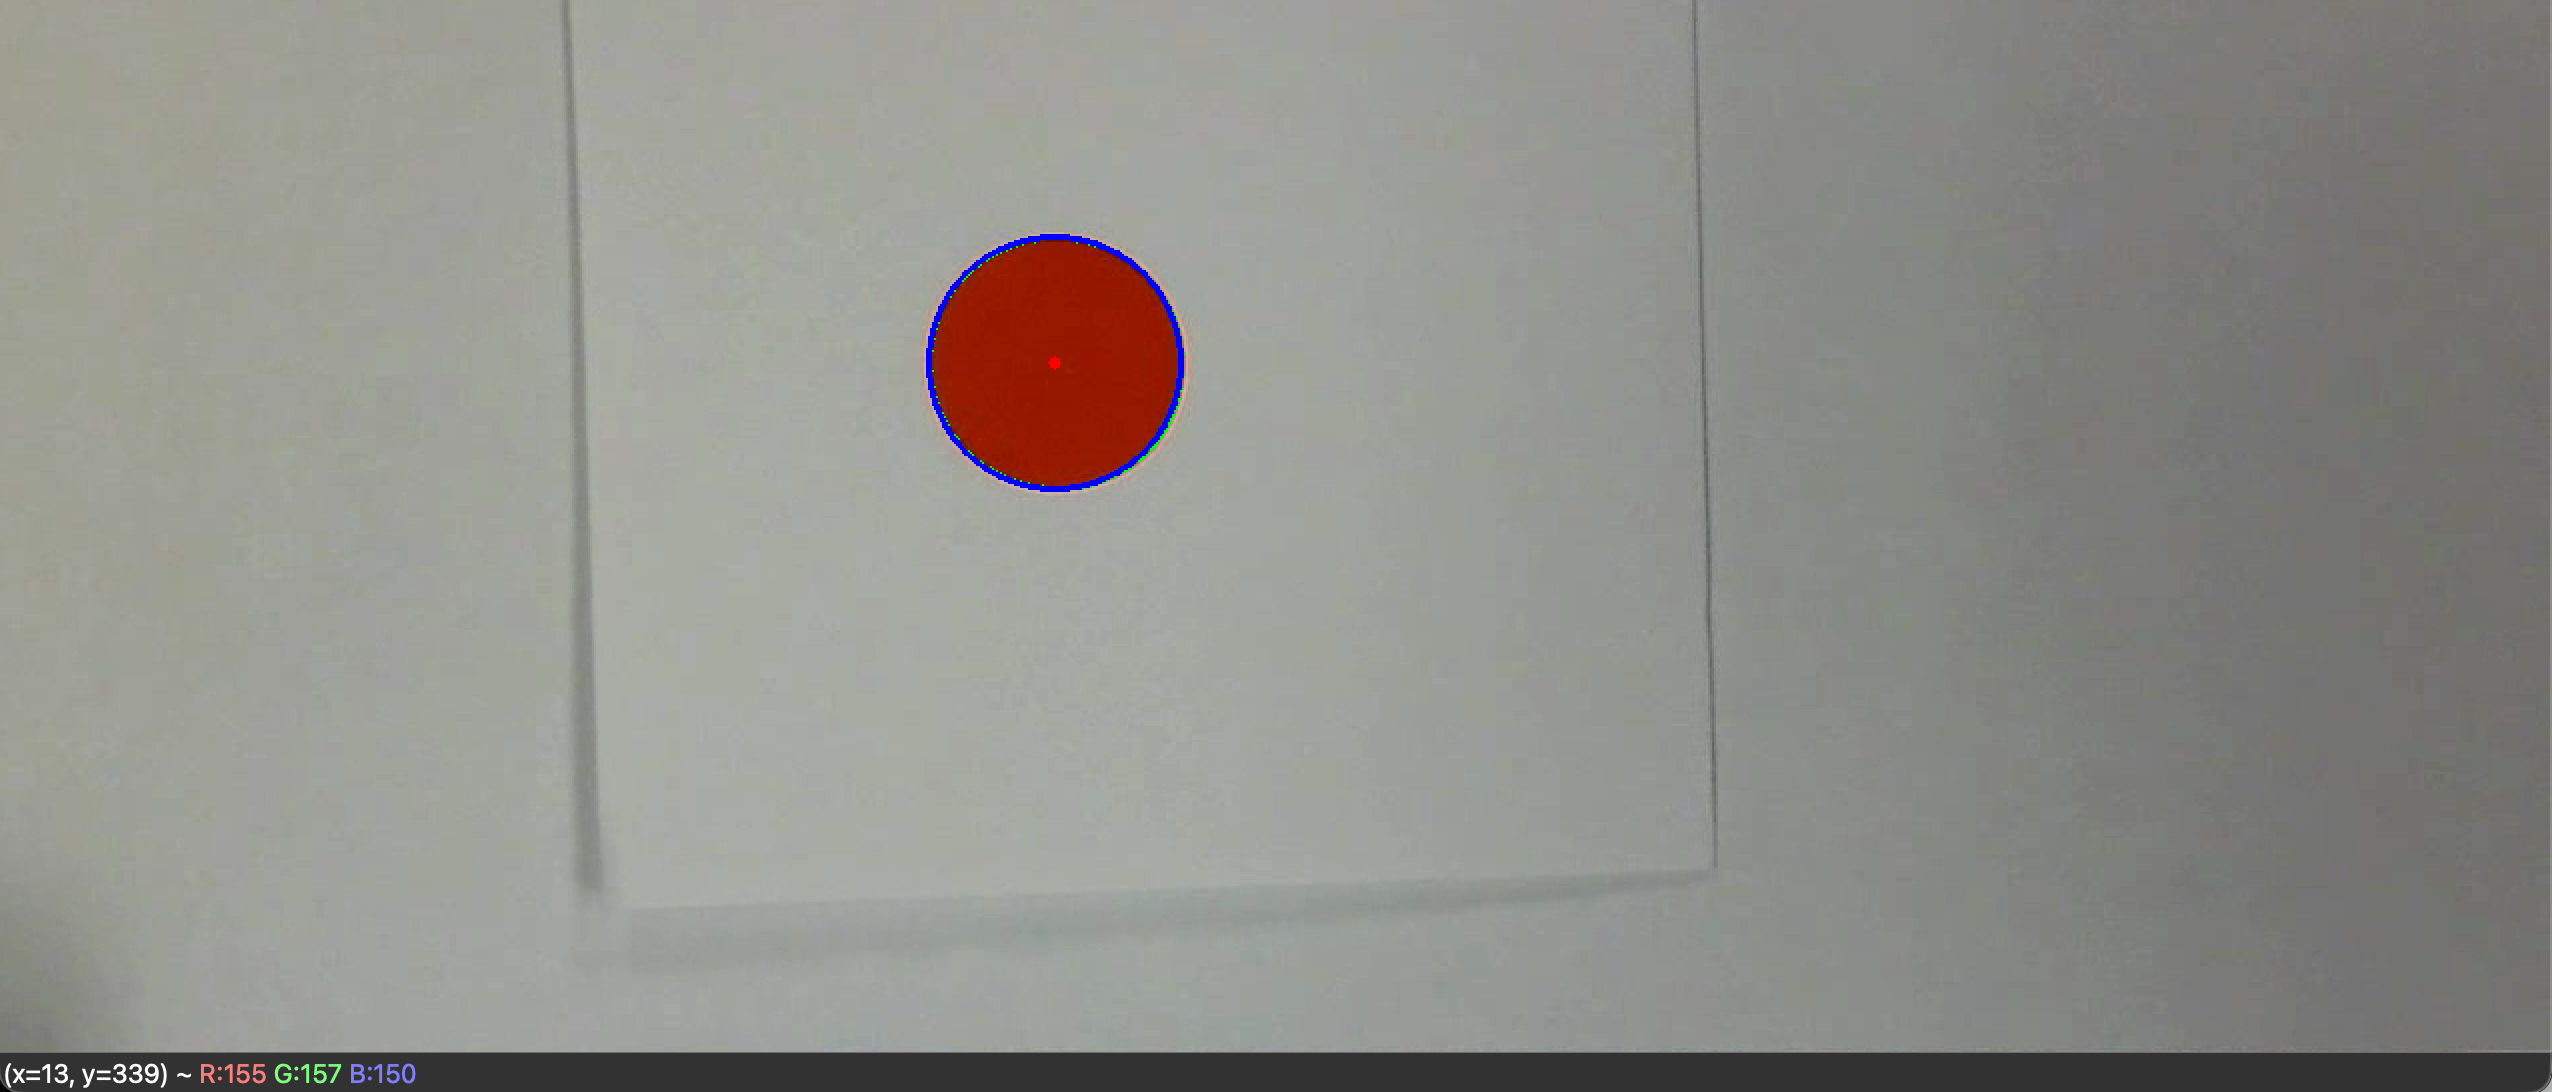
\includegraphics[width=0.75\linewidth]{images/recording_setup.png}
    \caption{Recording setup containing a single red dot on white paper over paper background, with the detected contour outline shown in blue.}
    \label{fig:setup}
\end{figure}

\subsection{Tracking Quality Assessment}

Figure 4 shows the tracked $(x,y)$ trajectory and $x$ versus time. The dot moved from about $(0.6,\,2.2)$\,in to $(8.5,\,3.4)$\,in over the recording, covering roughly 8.0\,in horizontally and rising about 1.2\,in vertically. The path is mostly smooth, with $y$ jitter of around $\pm 0.15$\,in throughout from moving the paper by hand.

In the $x$ versus time plot, Constant FPS (black), MSEC (green), and frame number (red) all reach $x \approx 8.5$\,in at $t \approx 35$\,s. The \texttt{time()} trace (blue) puts the same motion at $t \approx 45$\,s. The 10-second gap implies the camera averaged about $1{,}079/45 \approx 24$\,fps, not the 30\,fps assumed from the webcam specification. The frame-based methods compress the time axis and would overestimate velocity. For real-world velocity calculations, the \texttt{time()} function would be ideal.

\begin{figure}[H]
    \centering
    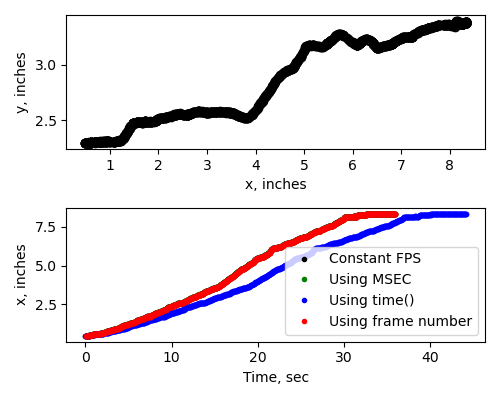
\includegraphics[width=0.75\linewidth]{figures/Trajectory_Plots.png}
    \caption{Top: tracked $(x,y)$ trajectory in inches. Bottom: $x$ position versus time using four timing methods. The \texttt{time()} trace (blue) extends to ${\approx}45$\,s while frame-based methods reach ${\approx}35$\,s.}
    \label{fig:trajectory}
\end{figure}

\newpage
\subsection{Ruler and Scale Comparison}

The pixel-to-inch conversion is computed as:

\begin{equation}
    \text{scale} = \frac{\text{ruler\_length}}{\text{width}} = \frac{9.5\,\text{in}}{1280\,\text{px}} \approx 0.00742\,\text{in/px}
    \label{eq:scale}
\end{equation}

\noindent This means one inch spans approximately 134.7 pixels. With this conversion, physical coordinates can be computed as:

\begin{align}
    x_\text{real} &= \text{scale} \cdot x_\text{px} \\
    y_\text{real} &= \text{scale} \cdot (\text{height} - y_\text{px})
\end{align}

\noindent where the height subtraction flips the $y$-axis so that positive $y$ points upward rather than downward which is used by image coordinates. Table 2 shows representative pixel-to-inch conversions at known ruler positions, verifying scale accuracy.

\begin{table}[H]
    \centering
    \caption{Representative Pixel-to-Inch Conversions Using Equation 12}
    \label{tab:scale_check}
    \begin{tabular}{ccc}
        \toprule
        \textbf{Pixel $x$} & \textbf{Computed $x$ [in]} & \textbf{Ruler Reference [in]} \\
        \midrule
        0     & 0.000 & 0.0 (left edge) \\
        135   & 1.002 & 1.0 \\
        270   & 2.004 & 2.0 \\
        640   & 4.750 & 4.75 (midpoint) \\
        1280  & 9.500 & 9.5 (right edge) \\
        \bottomrule
    \end{tabular}
\end{table}

\noindent The computed values match the ruler references to within 0.004\,in at the representative points, which is one pixel of rounding error. The main sources of measurement uncertainty are lens distortion, causing ruler lines to be non-uniformly spaced in pixel coordinates near the frame edges, and depth error, where any motion of the object toward or away from the camera changes its apparent scale relative to the fixed ruler, which could happen with an imperfectly flat setup. Slight tilting can introduce offsets that increase toward the edges of the frame.

\end{document}
